\documentclass{beamer}

\usepackage[italian]{babel}

\usetheme{default}

\author{Mirko Rossini, Thomas Fossati}
\title{KINK: integrazione semplice tra IoT e Internet}
\institute{UniBo, KoanLogic}

\begin{document}

\begin{frame}[plain]
  \titlepage
\end{frame}

\section{Internet of Things} 
% termine che indica una tecnologia, evoluzione di internet, per permettere la comunicazione macchina-macchina e macchina-uomo con enormi reti di oggetti
% c'è già (dal 2008, grazie a smartphone e tablet) e nel 2020 si raggiungerà quota 50 miliardi di apparecchi
\frame{\frametitle{Internet of Things} 
IoT: macchine interconnesse, anche senza interazione umana
\begin{figure}[h]
\centering
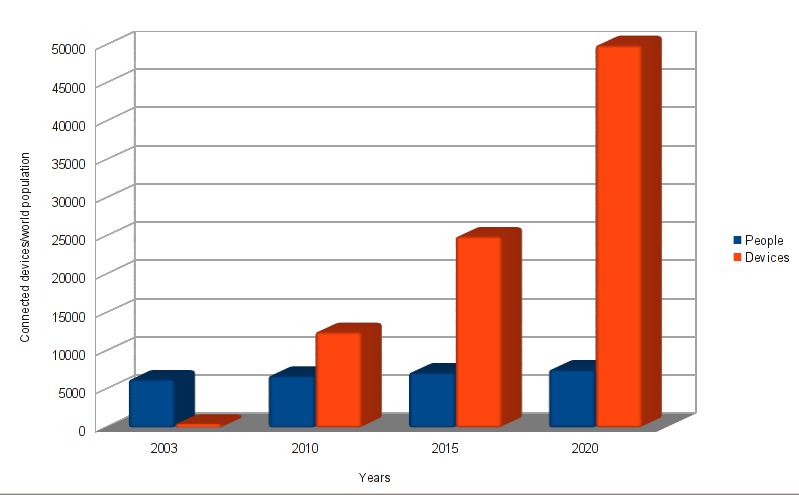
\includegraphics[width=1\textwidth]{imgs/iotpeoplevsdevices.png}
\label{fig:iotpeoplevsdevices}
\end{figure}

}
\frame{\frametitle{Applicazioni IoT}
\begin{itemize}
\item Domotica
\item Reti di sensori (allarme)
\item Smart grid
\item Ricerca
\end{itemize}
}
\frame{\frametitle{IoT: Difficolt\`{a} per lo sviluppo} 
\begin{itemize}
\item Energia
\item Standard e IPv6
\item Integrazione con internet
\end{itemize}
}
\frame{\frametitle{Gli standard IoT} 
\begin{itemize}
\item 802.15.4
\item 6LoWPAN
\item CoAP
\end{itemize}
}
\frame{\frametitle{Internet e IoT} 
\begin{figure}[h]
\centering
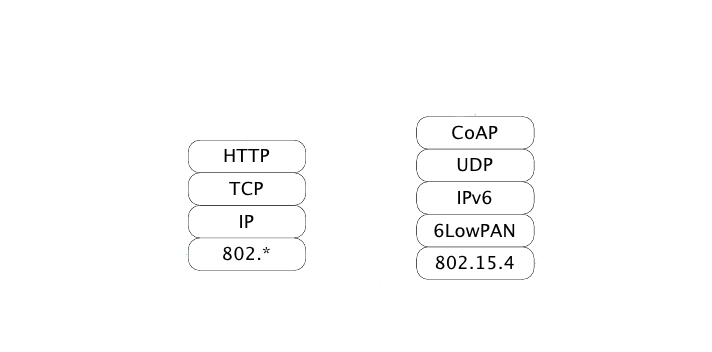
\includegraphics[width=1\textwidth]{imgs/stack-translation-nokink.png}
\label{fig:iotpeoplevsdevices}
\end{figure}
}
\frame{\frametitle{Kink} 
\begin{figure}[h]
\centering
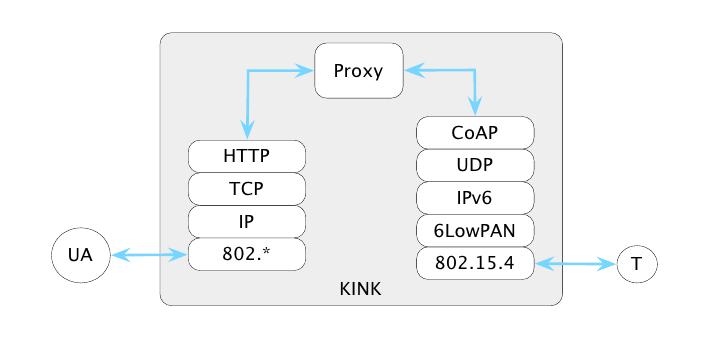
\includegraphics[width=1\textwidth]{imgs/stack-translation.png}
\label{fig:iotpeoplevsdevices}
\end{figure}
}
\frame{\frametitle{Particolarit\`{a} di CoAP} 
\begin{itemize}
\item Observe e uso per caching
\item Multicast
\item Link format
\item Trasporto datagram-oriented (UDP)
\end{itemize}
}

\frame{\frametitle{Vincoli} 
\begin{itemize}
\item Vicoli hardware derivanti dalla rete constrained
\item Modularit\`{a} e robustezza
\item Portabilit\`{a}
\end{itemize}

}
\frame{\frametitle{High level design} 
\begin{figure}[h]
\centering
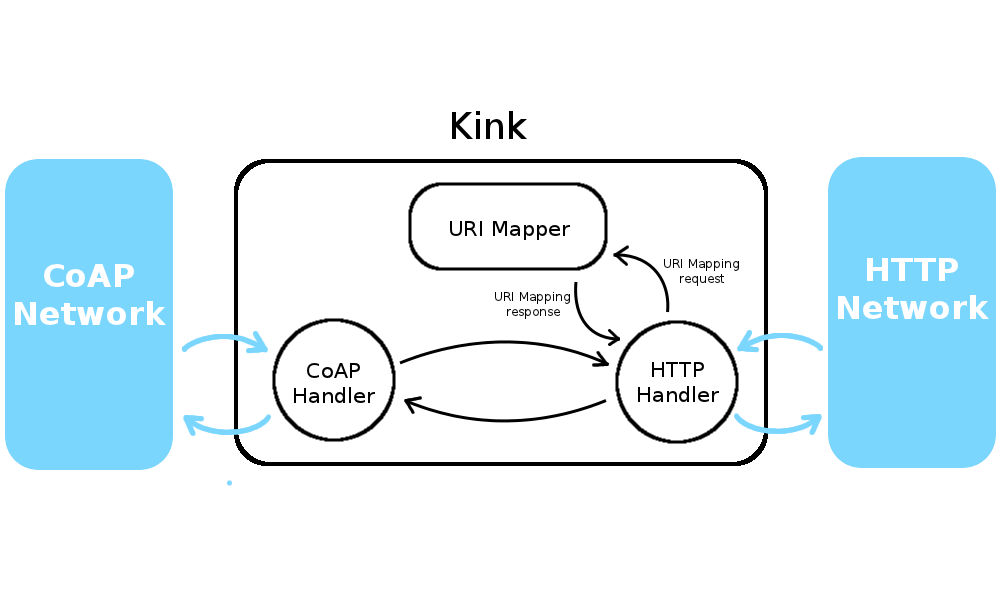
\includegraphics[width=1\textwidth]{imgs/high-level-design.png}
\label{fig:high-level-design}
\end{figure}

}
\frame{\frametitle{Low level design} 
\begin{figure}[h]
\centering
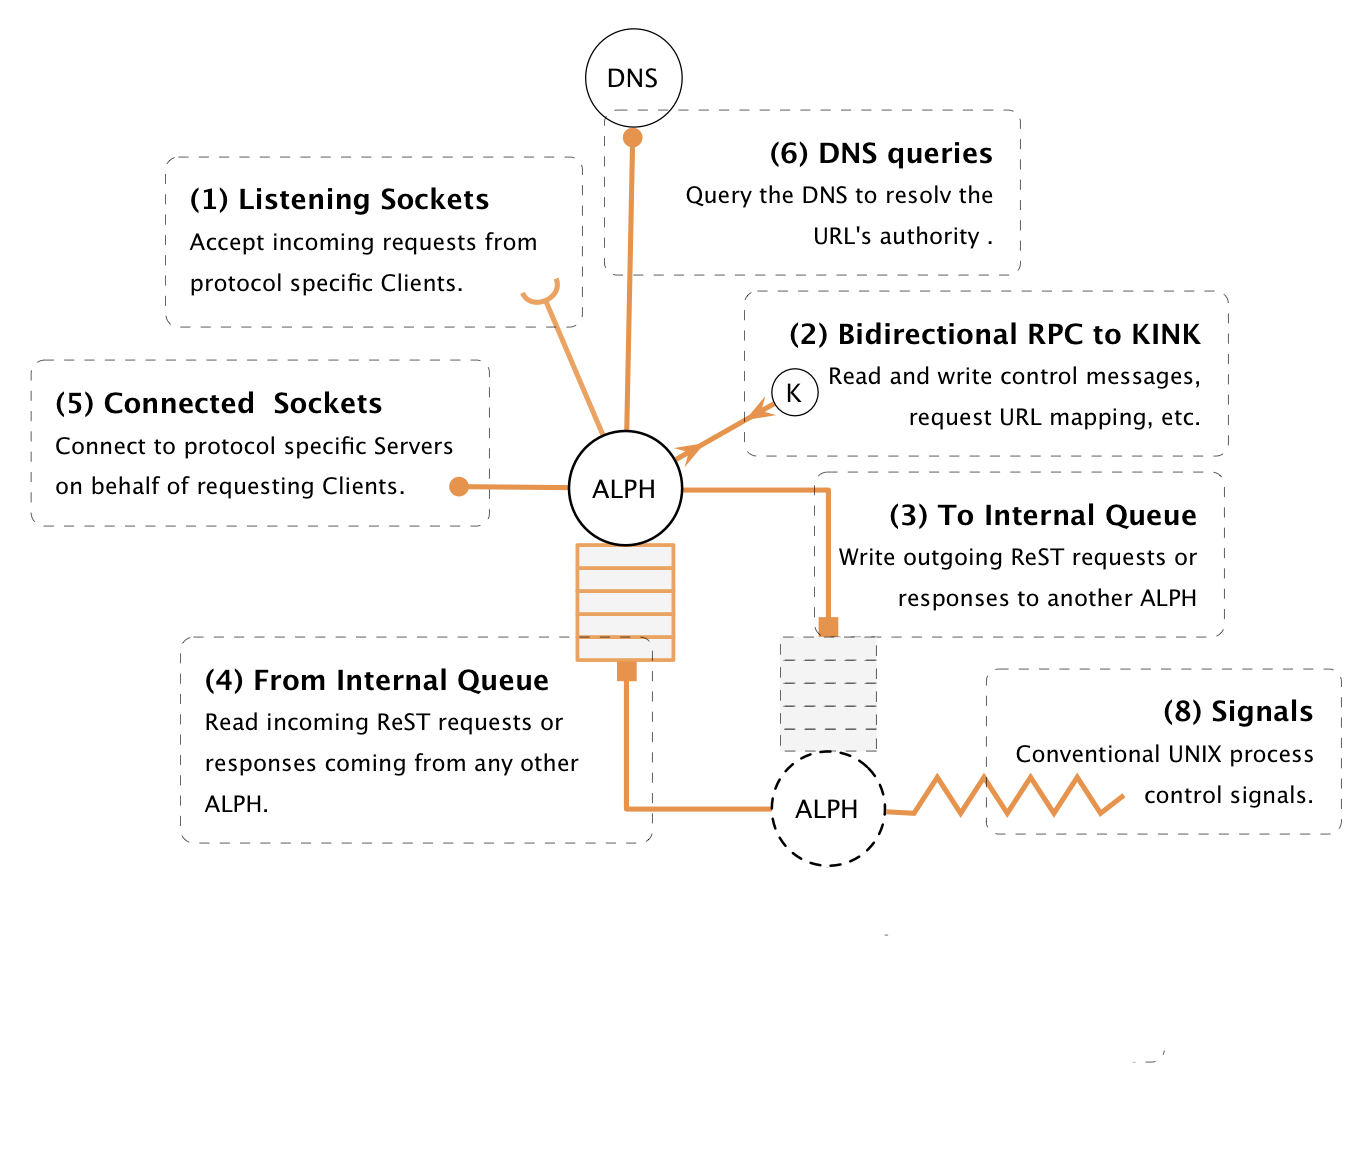
\includegraphics[width=1\textwidth]{imgs/kink-protocol-handler-anatomy.png}
\label{fig:kink-protocol-handler-anatomy}
\end{figure}
}
\section{Strumenti}
\frame{\frametitle{Strumenti necessari} 
\begin{itemize}
\item Caching
\item Implementazione HTTP
\item Implementazione CoAP
\item Longpoll per mapping di richieste observe
\end{itemize}

}
\frame{\frametitle{Strumenti scelti} 
\begin{itemize}
\item Estensione
\begin{itemize}
\item Apache
\item Varnish
\item Squid
\end{itemize}

\item Composizione
\begin{itemize}
\item libevent e il modulo evhttp
\item libev + libebb
\item Scelta dell'implementazione CoAP: libcoap e evcoap
\item POSIX mqueue
\end{itemize}
\end{itemize}
}
\section{Caching}
\frame{\frametitle{Caching: requisiti} 
\begin{itemize}
\item Agnostico: modulo comune a tutti i protocolli
\item Supporto per la validazione dei PDU
\item Dati statistici sulle richieste per ottimizzazione
\item Performance e basso impatto sulle risorse
\end{itemize}
 
}
\frame{\frametitle{Caching: scelte di design} 
% dati raggiungibili da due diversi protocol handlers
% evitare messaggistica lasciando i dati sul protocol handler che agisce come client
% update in caso di observe: se deve tornare sul protocol handler server, allora serve messaggistica
% potrebbe essere che se lo salva quando gli arriva, ma si duplicano i dati
% si potrebbe avere un unità centrale, ma comunque si dovrebbe creare un formato comune e fare lo stesso la traduzione
\begin{figure}[h]
\centering
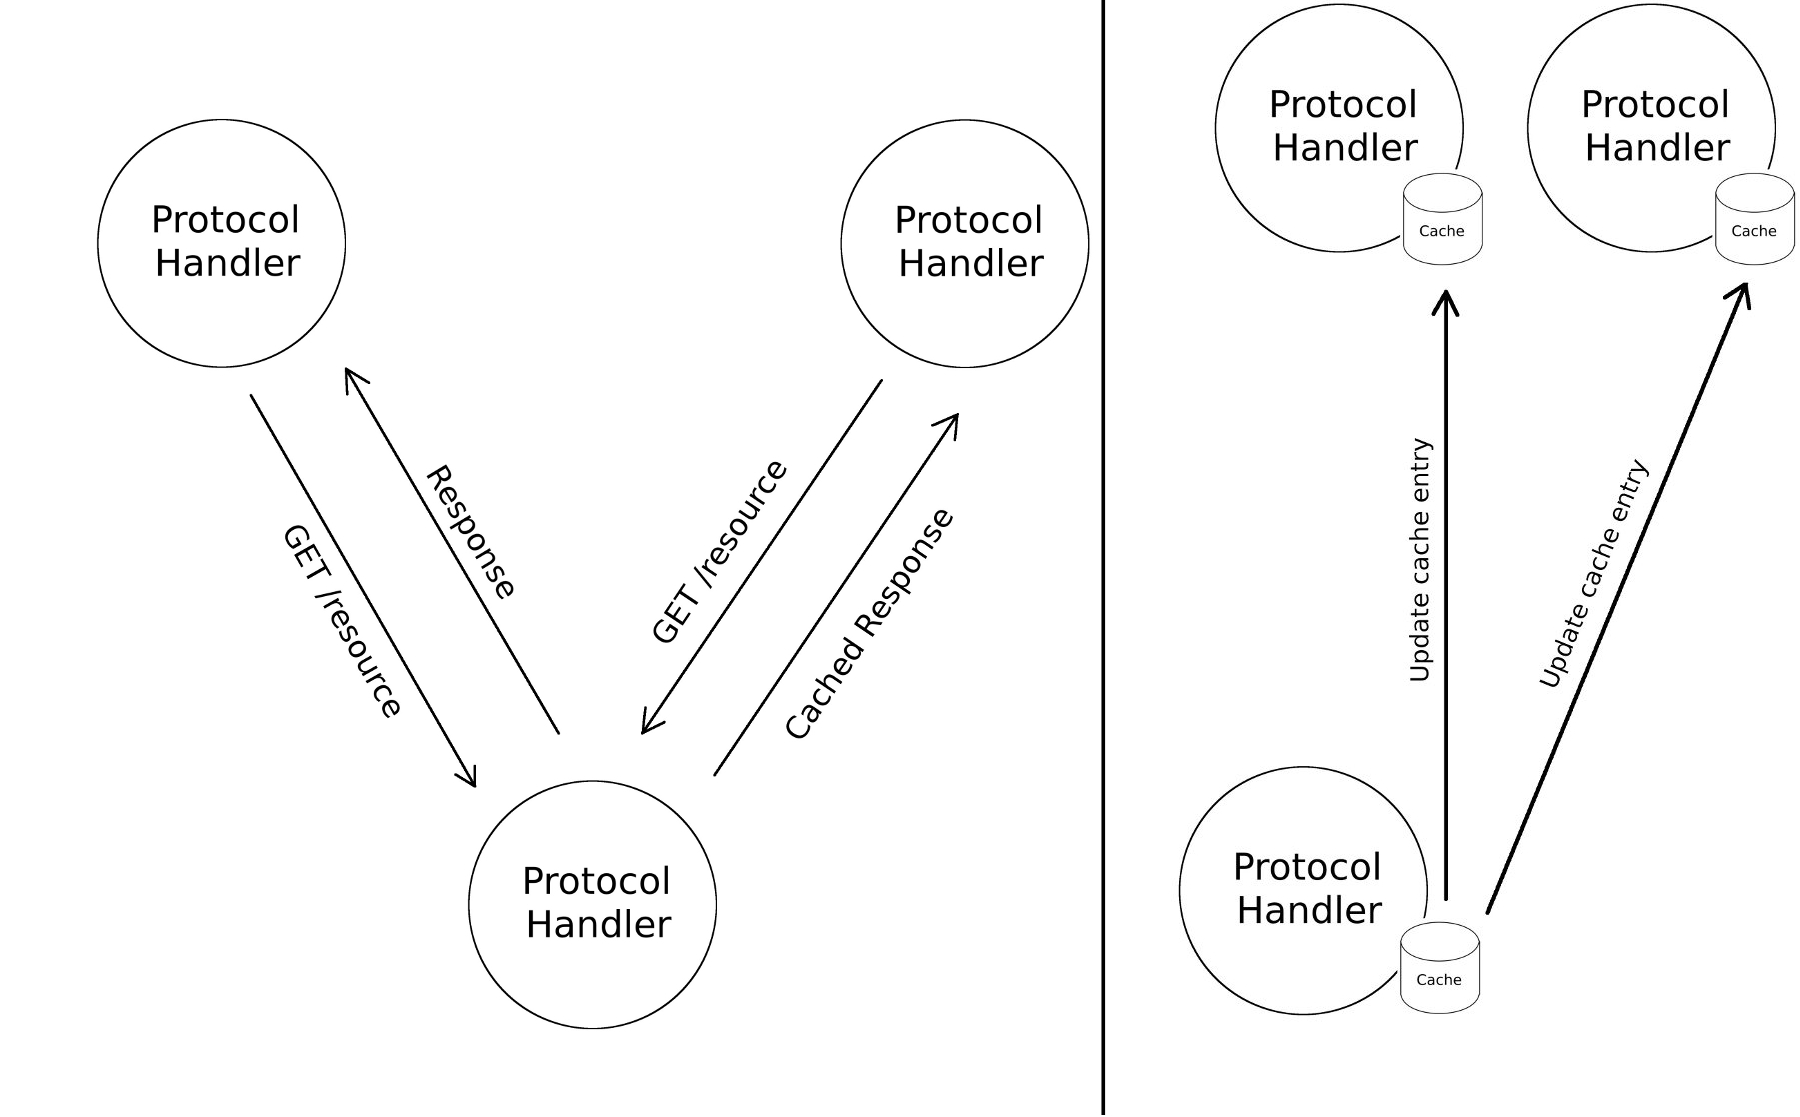
\includegraphics[width=1\textwidth]{imgs/cache_use_case.jpg}
\label{fig:cache_use_case}
\end{figure} 
}
\frame{\frametitle{Prossimi passi}
\begin{itemize}
  \item Proposte di modifica al protocollo: interazione tra sleepy nodes
  \begin{itemize}
    \item draft-giacomin-core-sleepy-option-00
    \item draft-fossati-core-publish-monitor-options-01
  \end{itemize}
  \item Distribuzione e feature aggiuntive
  \begin{itemize}
    \item Firmware basato su una distribuzione custom OpenWRT
    \item Immagine VM da utilizzare in data center per integrazione IoT - Internet
  \end{itemize}
\end{itemize}
 
}
\section{L'applicazione di test}
\frame{\frametitle{L'applicazione di test} 

\begin{columns}
  \begin{column}{0.5\textwidth}
    \begin{figure}[h]
    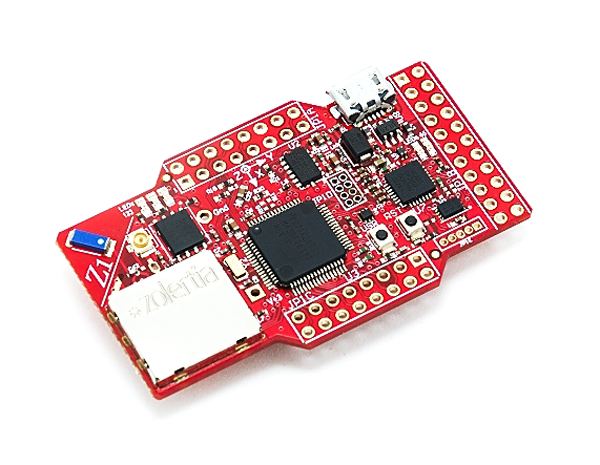
\includegraphics[width=1\textwidth]{imgs/Z1.png}
    \label{fig:z1}
    \end{figure} 
  \end{column}
  \begin{column}{0.5\textwidth}
    \begin{itemize}
      \item Sensori Z1
      \item Contiki
      \item RPL
    \end{itemize}
    
  \end{column}
\end{columns}
 
}
\frame{\frametitle{Demo} 
\begin{figure}[h]
\centering
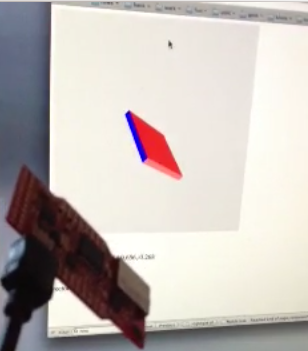
\includegraphics[width=0.6\textwidth]{imgs/demo-accel-2.png}
\label{fig:demo-accel-2}
\end{figure}

}

\end{document}
